The concepts illustrated in the previous chapters are now applied to a specific case: a dataframe of MC simulated single particles, which will be analysed in more detail in the next section.
		
		The reconstructed particles can be of two types:
		\begin{itemize}
			\item \textbf{single reconstruction}: when a particleis only reconstructed as electron or as photon;
			\item \textbf{double reconstruction}: when a particle cannot be classified in a single mode (el or ph) is reconstructed in both modes and is called \textit{ambiguous}. The final classification is
		\end{itemize}
		
		In this second case the ML applies. A supervised machine learning (Gradient BDT) is used to create and train a model. Then this model is applied to the double reconstruction to classify electrons and photons and increase the reconstruction efficiency.
		%Let's see how this BDT is created
		
		\section{Dataframe and BDT training}
			\subsection{Dataframe}
			
			\subsection{Discriminating features}
				In order to create a good model, the choice of the features it will have to work on is crucial. The most useful characteristics are those that present the greatest differences between photons and electrons, which are therefore more discriminating. It is also important to use features that guarantee the generality of the model.The features can be divided into two categories: electron and photon features.
				\subsubsection{Electron features}
				Electron features are those that characterize the particles reconstructed as electrons. Electrons have many hits in the first layers of detectors, as opposed to photons. This is because the most part of photons is still unconverted. So electron reconstructed as electrons (tur\_el/reco\_el) should have more hits than photons reconstructed as electrons (true\_ph/reco\_el). This can be seen in the characteristics 'el\_track\_hasInnermostHits' (a boolean, which says if the particle has hit the first expected layer or not), 'el\_trkPixelHits' (a pixel hit counter), 'el\_trkSiHits'(a silicon hit counter) shown in the figure \ref{fig:el_hit}.
				\begin{figure}
					\centering
					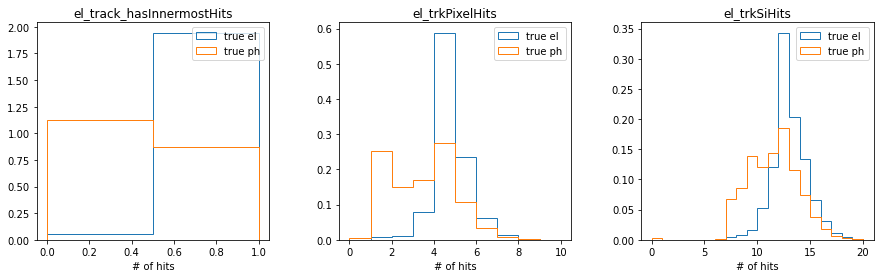
\includegraphics[width=0.7\textheight]{tesi_images/el_hit.png}
					\caption{}
					\label{fig:el_hit}
				\end{figure}
				
				The track quality, as it is determinated from the pixel and SCT hits, is different in the two cases therefore the physics quantities reconstructed from the track. This quantities (plots in Figure \ref{fig:el_physics_quantities}) are:
				\begin{itemize}
					\item 'el\_track\_ep',
					\item 'el\_trackz0',
					\item 'el\_cl\_pt, 
					\item 'el\_cl\_eta'
				\end{itemize}
			
				\begin{figure}
					\centering
					\subfloat[]{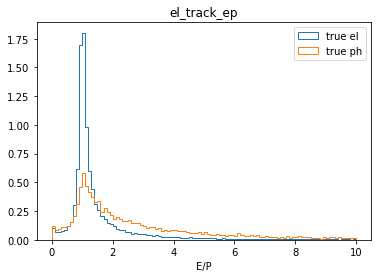
\includegraphics[width=.44\textwidth]{tesi_images/el_track_ep.png}} \quad
					\subfloat[]{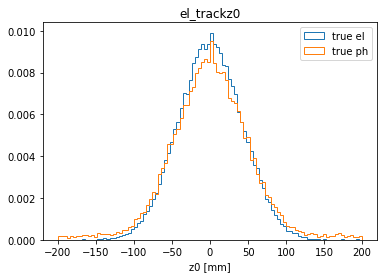
\includegraphics[width=.45\textwidth]{tesi_images/el_trackz0.png}}
					\newline
					\subfloat[]{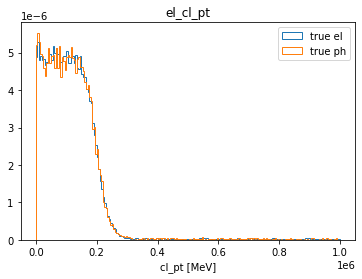
\includegraphics[width=.44\textwidth]{tesi_images/el_cl_pt.png}} \quad
					\subfloat[]{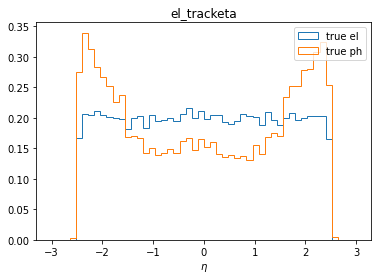
\includegraphics[width=.44\textwidth]{tesi_images/el_tracketa.png}}
					\caption{Electron physics quantities reconstructed from the track}
					\label{fig:el_physics_quantities}
				\end{figure}
				
				
				
				\subsubsection{Photon features}
				As electron, the photon quality track (of the pair $e^{+}e^{-}$) is discriminating and therefore also the Pixel/SCT hits and $p_t$.
				
				Other useful photon features for classification are those related to conversion:
				\begin{itemize}
					\item \textbf{'ph\_zconv'} and \textbf{'ph\_Rconv'}:these characteristics contain information of the conversion point in the coordinates R and z. True\_el/reco\_ph have a conversion point close to the point of interaction as their track starts from the beginning.
					\item \textbf{'ph\_pt1conv'}, \textbf{'ph\_pt2conv'} and \textbf{'ph\_ptconv'}. All these three features have been scaled with 'ph\_cl\_pt' to eliminate all kinematics information 
					\item \textbf{'pt1conv/ptconv'} contains information on conversion symmetry. This characteristic for true\_el/reco\_ph tends to 1, since most of them have a single track.
				\end{itemize}
				
			\section{Parameters and Hyperparameter optimization}	
			In order to create a good predictive model, the choice of parameters is crucial, therefore the hyperparameter optimization is used. Hyperparameters are LGMB adjustable parameters chosen for the training of a model, which regulate the training process. 
			
			The objective of the hyperparameter optimization is to search the various configurations of the hyperparameters, contained in the hyperparameter space, to find a configuration with the best performance. The hyperparameter space consists of two types of hyperparameters: discrete or continuous. Let's focus on the continuous ones.
			Continuous hyperparameters are specified as a uniform distribution   over a continuous range. 
			
			So after defining the space of the hyperparameters, we move on to the search for the best configuration. This search can be of various types:
			\begin{itemize}
				\item \textbf{random search}: in random search the hyperparameter values are randomly selected from the defined search space. It allows the  hyperparameter space to include both discrete and continuous hyperparameters;
				\item \textbf{grind search}: grid sampling performs a simple grid search on all possible values in the defined search space;
				\item \textbf{bayesian search}: bayesian sampling uses the knowledge of the previous samplings when choosing hyperparameter values, effectively attempting to improve the reported primary metric. The sample is selected based on the performance of the previous sample, so that the new sample improves the primary metric reported. 
			\end{itemize}
			The bayesian search is used by the Python library \textit{Hyperopt}, which is implemented in the code in order to perform the optimization.
			
			The training parameters are listed in the Table \ref{tab:parameters} and the ones that have been optimized are:
			\begin{itemize}
				\item \textbf{bagging}: in bagging, several models of the same type are trained on different datasets (aggregation, typical of ensemble learning), each obtained from the initial dataset by random sampling with replacement (bootstrap).
				\item \textbf{number of leaves}: it is the maximum number of leaves,that a tree could have. It is useful to avoid overfitting.
				\item \textbf{feature fraction}: it is used when boosting is random forest. 0.82 feature fraction means LightGBM will used 82\% of parameters randomly in each iteration for building trees.
				\item \textbf{learning rate}: it determines the effect of each tree on the final outcome.
			\end{itemize}
			Durante hyperparam sono state utilizzate 200 ricerche
			
			\begin{table}
				\centering
				\begin{tabular}{cc}
					\toprule[1.5pt]
					Parameter & Value\\
					\midrule
					Metric & xentropy \\
					Objective & xentropy \\
					Bagging seed & 42 \\
					Feature fraction seed & 42 \\
					Is unbalance & True \\
					Number of leaves & 70 \\
					Feature fraction & 0.8279495901643081 \\
					Bagging & 0.8039490145162762 \\
					Learning rate & 0.06057403872801198 \\
					\bottomrule[1.5pt]
				\end{tabular}
				\caption{Parameters used in the model's training}
				\label{tab:parameters}
			\end{table}